%!TEX root = ../Thesis.tex

\section{Benchmark problems}\label{sec: Experimental work: Benchmarking}
\subsection{Supervised learning benchmark}
Within the supervised learning setting, the classical problem of handwritten digit recognition based on the \gls{MNIST} dataset \cite{LeCun1998} was chosen. This is a small and relatively simple data set that has allowed for rapid prototyping and aided in algorithm development, historically and in this thesis. Even though it has recently received criticism for being too simple, it remains one of the most widely used benchmarks within deep learning \cite{Xiao2017}. The training data consists of 60.000 greyscale images of handwritten digits between 0 and 9 and the associated label. Each image has $28\times28$ pixels and represents a single digit. The test data consists of 10.000 images and associated labels.
In this thesis, no data augmentation has been applied to the data set. Examples from the \gls{MNIST} dataset can be seen in \autoref{fig: mnist-examples/MNIST-10x10-sorted.pdf}.
\begin{figure}[tbp!]
    \centering
    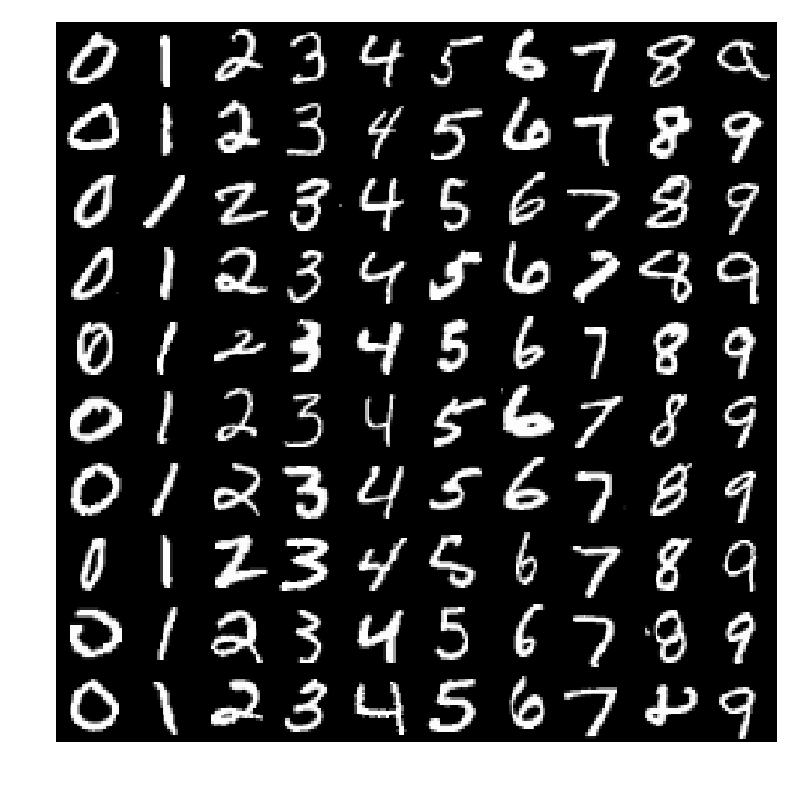
\includegraphics[width=0.60\textwidth]{graphics/mnist-examples/MNIST-10x10-sorted.pdf}
    \caption{
        Examples from the \gls{MNIST} dataset sorted by target values from 0 on the left and 9 on the right. As is well-known, a few examples from the dataset are very hard to correctly classify, note for example the bottom most 8 and the top most 9.
    }
    \label{fig: mnist-examples/MNIST-10x10-sorted.pdf}
\end{figure}

To the author's best knowledge, the currently best performing non-ensemble \gls{NN} model on \gls{MNIST} is the deep \gls{FNN} using DropConnect \cite{Wan2013, Hasanpour2016} which achieved $99.79\%$ classification accuracy also exploiting extreme data augmentation. An accuracy of $99.76\%$ was achieved in \cite{Chang2015} which uses a max-out network in network \cite{Lin2013} model with no data augmentation. Using backpropagation and the network to be used for \gls{MNIST} in this thesis (introduced in \autoref{sec: Experimental work: Neural network architectures (MNIST)} and shown in \autoref{lst: Network models: MNIST with batch normalization}) the best achievable accuracy is about $99.1\%$ using \gls{SGD} with momentum training for 20 epochs. With the Adam algorithm, accuracy can reach $99.2\%$ for 20 epochs.


\subsection{Reinforcement learning benchmarks}
Within the reinforcement learning setting, focus has been primarily on two environments from the OpenAI Gym toolkit \cite{Brockman2016}. The first environment is the Atari-2600 game of Freeway\footnote{\url{http://en.wikipedia.org/wiki/Freeway_(video_game)}, \url{http://gym.openai.com/envs/Freeway-v0/}} in which the agent controls a chicken that must be brought to pass a busy ten lane highway by moving either up or down. If hit by a car, the chicken is pushed either slightly back or moved to the starting position. A reward of $1$ is given for each successful passage and the total score is the number of passages within a time slot of $2$ minutes and $16$ seconds. In \cite{Salimans2017}, using a the fixed variance \gls{ES} similar to \gls{VO}, a score of $31$ was achieved when averaged over 10 re-runs with the DQN network of \cite{Mnih2016} encoding a deterministic policy. This network is also used for \gls{RL} in this thesis

The second \gls{RL} environment is the Atari game of Seaquest\footnote{\url{http://en.wikipedia.org/wiki/Seaquest_(video_game)}, \url{http://gym.openai.com/envs/Seaquest-v0/}}. Here, the agent controls a submarine which must fend off enemies using torpedoes while rescuing divers by moving to their location. The submarine's oxygen supply is limited and the agent must occasionally bring it to the surface to refill and to receive points from rescued divers. The submarine can move in four directions and fire torpedoes. Seaquest is considered harder than Freeway due to the larger action space and more complicated objective. In \cite{Salimans2017}, a score of $1390.0$ was achieved in the same way as for Freeway.

In this thesis, \gls{VO} is used to optimize a policy which maps from the environment's observation space to its action space. The policy is parameterized by a \gls{NN} model, in this case also called a policy network \cite{Silver2014}. The policy is deterministic in that the most probable action, as computed by the policy network, is always taken. Due to computational limitations, the number of experiments made in the reinforcement setting is fewer than in the supervised setting.

In general, hyperparameter optimization has been performed manually and heuristically. Ideally, random hyperparameter search \cite{Bergstra2012a} would have been employed to find optimal hyperparameters but was not due to limited computational resources.


\subsection{Preprocessing of MNIST}
Although no data augmentation is applied to the \gls{MNIST} dataset, the data is normalized before being input to the \gls{NN}. That is, for each digit image, the average pixel value is computed along with the variance and these are aggregated to a mean and variance for the full dataset. For \gls{MNIST}, this could be done in a single computation since the entire data set fits in memory. However, since larger datasets were also tried out, the computation was implemented in an online manner according to the algorithm proposed by \cite{Welford1962}. 

The algorithm consists of updating the mean as usual and the variance through online updates to the squared sample distance from the mean. For the mean
\begin{equation}
    \bar{x}_n = \bar{x}_{n-1} + \frac{x_n-\bar{x}_{n-1}}{n} \ .
\end{equation}
% \begin{align*}
%     \bar{x}_n
%     &= \frac{1}{n}\sum_{i=1}^n x_i\\
%     %&= \frac{1}{n}\pa{\sum_{i=1}^{n-1} x_i + x_n}\\
%     &= \frac{n-1}{n}\frac{1}{n-1}\sum_{i=1}^{n-1} x_i + \frac{1}{n}x_n\\
%     &= \frac{n-1}{n}\bar{x}_{n-1} + \frac{1}{n}x_n\\
%     &= \bar{x}_{n-1} + \frac{x_n-\bar{x}_{n-1}}{n} \ .
% \end{align*}
%which can be written as
%\begin{equation}
%    \bar{x}_n = \bar{x}_{n-1} + \frac{x_n-\bar{x}_{n-1}}{n} \ .
%\end{equation}
Likewise, the update for the variance is
\begin{align*}
    s^2_n
    &= \frac{(n-2)}{(n-1)} s^2_{n-1} + \frac{(x_n - \bar{x}_{n-1})^2}{n} \ , \quad n>1 \ .
\end{align*}
This online update of the variance is prone to numerical instability which is avoided by updating the squared sample distance from the mean
\begin{equation*}
    M_{2,n} = M_{2,n-1} + (x_n - \bar{x}_{n})^2 %(x_n - \bar{x}_{n-1})(x_n - \bar{x}_{n})
\end{equation*}
and then computing 
\begin{equation*}
    s_n^2 = \frac{M_{2,n}}{n-1} \ .
\end{equation*}
These formulas have been generalized to the case of multiple examples being added at each online update \cite{Chan1979}. Here, this is needed to avoid looping over the $28\times28=784$ pixels of each image. Let $A$ and $B$ denote two samples with $n_A$ and $n_B$ examples respectively and a mean, variance and squared sample distance from the mean denoted by $\bar{x}_A$, $\bar{x}_B$, $s^2_A$, $s^2_B$, $M_{2,A}$, $M_{2,B}$, respectively. The update formulas for the aggregated sample $X$ are then
\begin{align*}
    \delta &= \bar{x}_B - \bar{x}_A\\
    \bar{x}_X &= \frac{n_A}{n_X}\bar{x}_A + \frac{n_B}{n_X}\bar{x}_B\\
    M_{2,X} &= M_{2,A} + M_{2,B} + \delta^2\frac{n_A n_B}{n_X}\\
    s_X^2 &= \frac{M_{2,X}}{n_X-1}
\end{align*}
where $n_X = n_A + n_B$.

The computed mean and standard deviation for the \gls{MNIST} dataset were then used to normalize each input pixel $x_i$ as
\begin{equation*}
    \hat{x}_i = \frac{x_i-\bar{x}}{s} \ .
\end{equation*}


\subsection{Preprocessing of Atari environments} \label{sec: Experimental section: Preprocessing of Atari environments}
Atari environments are preprocessed in the same way as in \cite{Mnih2015}. A frame from an Atari game is a $210\times160\times3$ pixels RGB image. Due to the limited number of sprites an Atari 2600 was able to display at once, some objects in games occur only in even frames while others occur only in odd frames \cite{Mnih2015}. To remove this flickering, a single frame is encoded as the maximum value of each pixel of the most recent frame and the previous frame. The frame is then converted to greyscale and resized to $84\times84$ using a pixel area relation which gives moiré-free results, is fast and yields good results for image downsampling \cite{OpenCVDevelopmentTeam2014}. This reduces the dimensionality of the frame by more than a factor of ten from $210\times160\times3=100800$ pixels to $84\times84=7056$ pixels. The input given to the \gls{NN} model is the four most recent frames seen such that the input dimension is $4\times84\times84$. This gives the model directional information about movement in the images without the use of recurrent units.

\begin{figure}[tbp!]
    \begin{subfigure}[b]{0.32\textwidth}
        \centering
        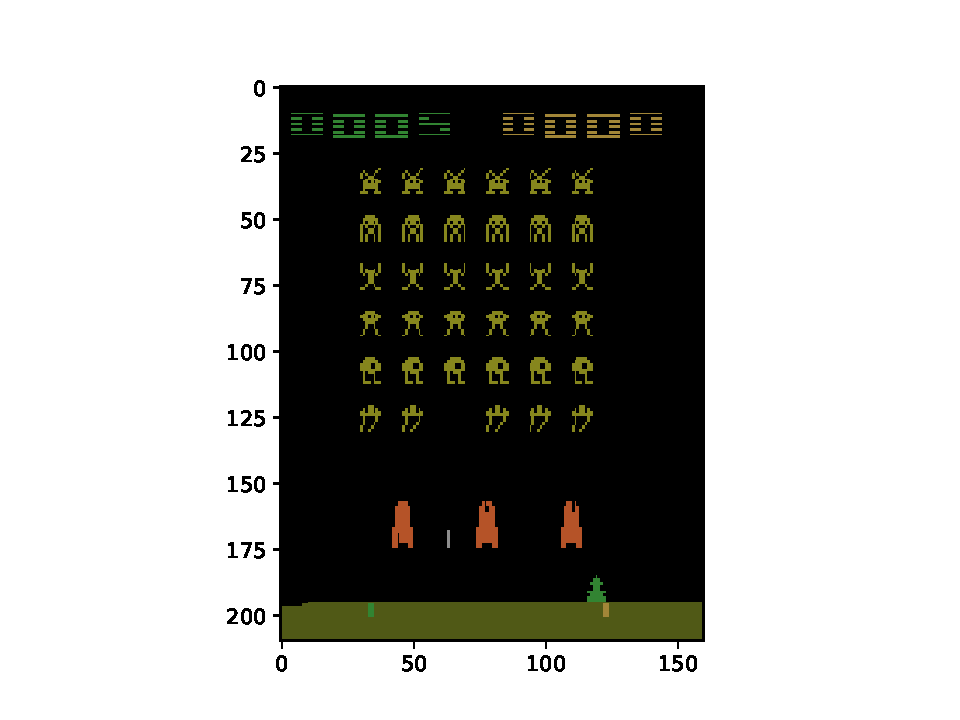
\includegraphics[height=5.8cm]{graphics/atari-pre-processing/1-spaceinvaders-original-cropped.pdf}
        \caption{}
        \label{fig: Experimental work: atari-pre-processing-1-spaceinvaders-original}
    \end{subfigure}
    \hfill
    \begin{subfigure}[b]{0.32\textwidth}
        \centering
        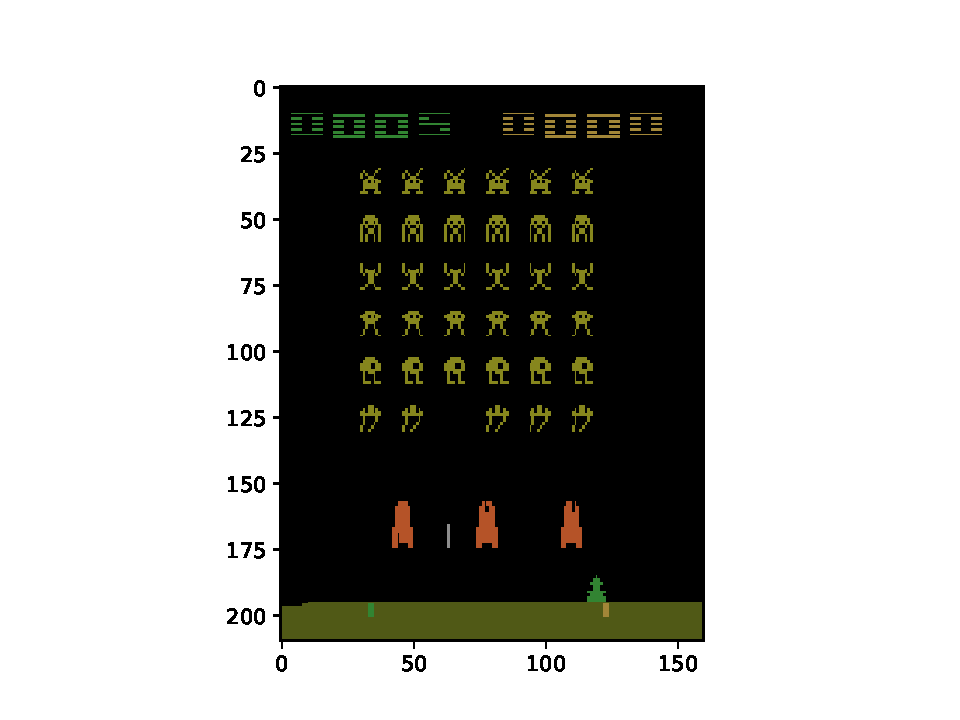
\includegraphics[height=5.8cm]{graphics/atari-pre-processing/2-spaceinvaders-flicker-cropped.pdf}
        \caption{}
    \label{fig: Experimental work: atari-pre-processing-2-spaceinvaders-flicker}
    \end{subfigure}
    \hfill
    \begin{subfigure}[b]{0.32\textwidth}
        \centering
        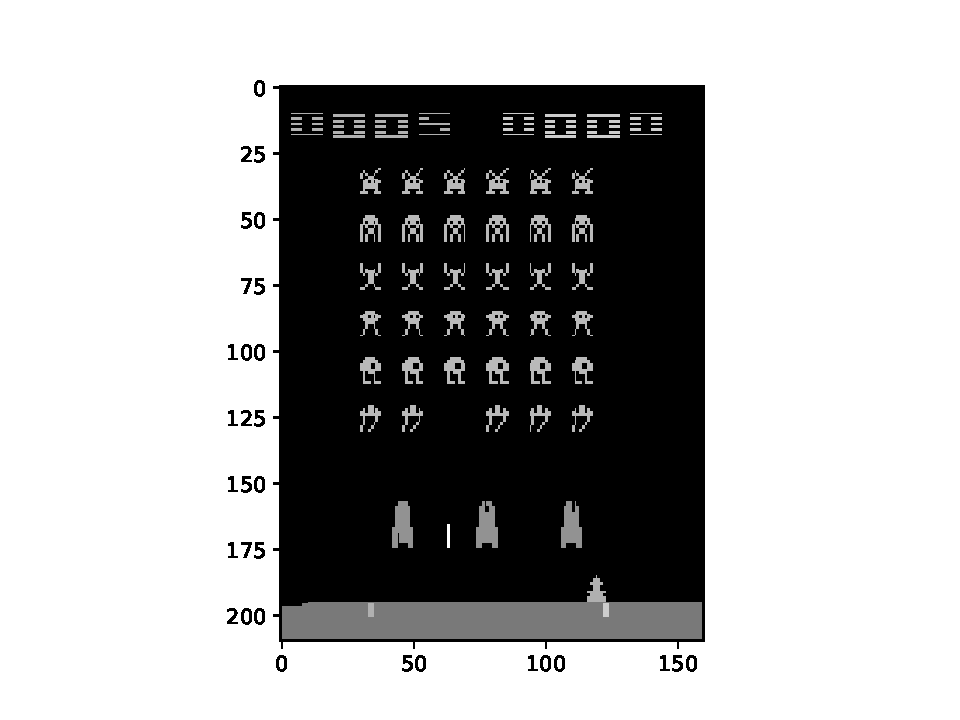
\includegraphics[height=5.8cm]{graphics/atari-pre-processing/3-spaceinvaders-grey-cropped.pdf}
        \caption{}
        \label{fig: Experimental work: atari-pre-processing-3-spaceinvaders-grey}
    \end{subfigure}
    \centering
    \begin{subfigure}[b]{0.40\textwidth}
        \centering
        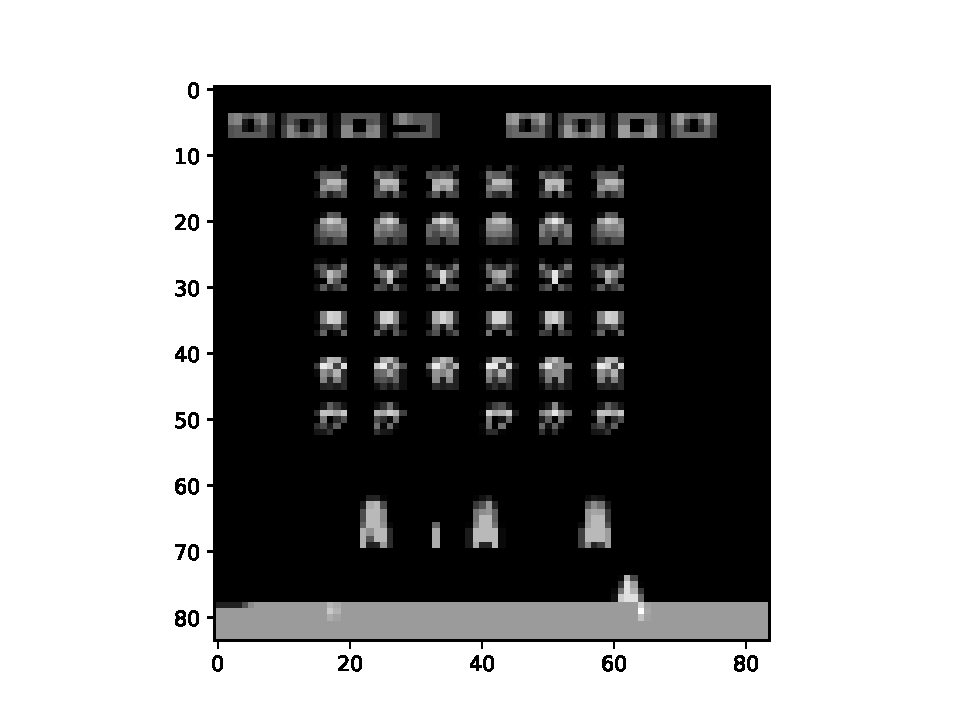
\includegraphics[height=5.8cm]{graphics/atari-pre-processing/4-spaceinvaders-resized-cropped.pdf}
        \caption{}
        \label{fig: Experimental work: atari-pre-processing-4-spaceinvaders-resized}
    \end{subfigure}
    \caption{\subref{fig: Experimental work: atari-pre-processing-1-spaceinvaders-original} Original frame from Space Invaders. \subref{fig: Experimental work: atari-pre-processing-2-spaceinvaders-flicker} Flicker removed by setting pixels to their maximal value over previous four frames. Notice the elongated beam. \subref{fig: Experimental work: atari-pre-processing-3-spaceinvaders-grey} Converted to greyscale. \subref{fig: Experimental work: atari-pre-processing-4-spaceinvaders-resized} Resized to $84\times84$.}
    \label{fig: Experimental work: atari-pre-processing}
\end{figure}

An illustration of the results of this preprocessing can be seen for the game of Space Invaders in \autoref{fig: Experimental work: atari-pre-processing}. Note that the fired beam is longer in \subref{fig: Experimental work: atari-pre-processing-2-spaceinvaders-flicker} compared to \subref{fig: Experimental work: atari-pre-processing-1-spaceinvaders-original}. This is a side effect of combining successive images by pixel maximum which slightly elongates moving objects.
